\documentclass[a4paper,12pt]{article}
\usepackage[italian]{babel}
\usepackage[utf8]{inputenc}
\usepackage{graphicx} %per aggiungere le immagini
\usepackage{listings} %per aggiungere codice sorgente
\usepackage{tabularx}
\usepackage{amsmath}

\lstset{basicstyle=\ttfamily\footnotesize,breaklines=true}

% interruzione di pagina tra le section
\let\oldsection\section
\renewcommand\section{\clearpage\oldsection}

% \newenvironment{cypher}{\begin{lstlisting}[keepspaces=true]}{\end{lstlisting}}

\title{Tesi di Laurea}
\author{Lorenzo Gabriele}

\pagenumbering{arabic}
\linespread{1.25}
\begin{document}

\maketitle
\clearpage
\tableofcontents
\clearpage

\section{Introduzione}

\section{Motivazioni}



\subsection{Formato dei dati}
Per poter effettuare lo studio era necessario lavorare su dati reali. Una stima della qualità degli autori di testi accademici con la pretesa di essere più efficace a stimare la effettiva rilevanza, deve essere valorata da dati reali, possibilmente in numero sufficiente affinché siano considerabili statisticamente rilevanti.
\par
In un primo momento si è pensato di utilizzare, come fonte da cui ricavare i dati, un servizio on-line di consultazione degli articoli come Scopus. \\ 
La maniera di ottenere i dati sarebbe dovuta essere incrementale.
Per incrementale si intende il non costuire l'intero dataset a priori dell'analisi dei nodi del grafo, bensì costruire il sotto-grafo "centrato" rispetto ad un autore.
Quindi, scegliendo un autore, si analizzano i suoi articoli, le referenze di tali articoli, ed infine dagli autori delle referenze è possibile stabilire un collegamento tra i due autori. \\
L'approccio descritto possiede almeno due aspetti negativi non trascurabili,
La procedura ha una complessità elevata e richiede una ripetutamente l'interrogazione di un servizio online, quale Scopus, che vieta espressamente le pratiche di Data Mining attraverso l'utilizzo delle loro API. \\
Dunque si è cercata una strada differente che permettesse di analizzare localmente una grande quantità di dati.
\par
Come scelta definitiva si è utilizzato un dataset ospitato dal sito aminer.org. Tale sito si prefige l'obiettivo di riunire i dati di quanti più articoli possibili, relativamente a pubblicazioni del macro-ambito della computer science. \\
aminer.org aggiorna ogni anno il suo dataset, rilasciandone una nuova versione. Nella versione 10 (la versione di cui si fa riferimento in questo lavoro) possiede un numero di poco superiore ai 3 milioni di articoli. \\
\begin{figure}[h!]
  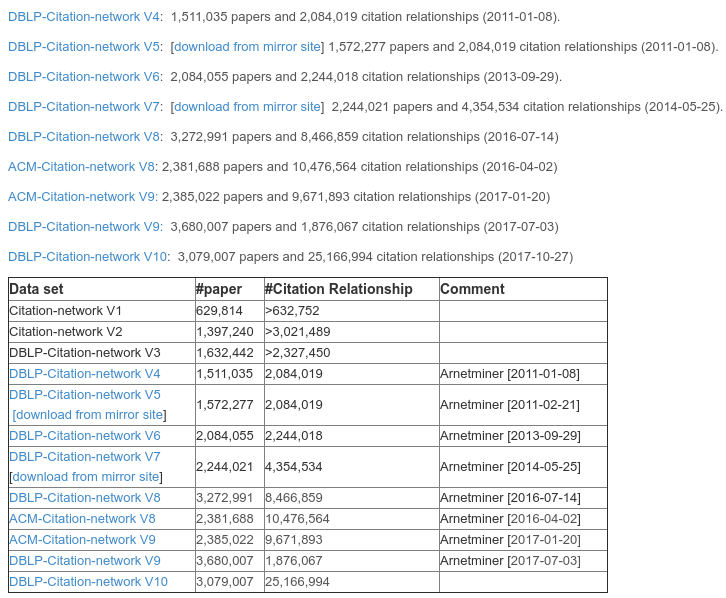
\includegraphics[width=\linewidth]{images/aminer.jpg}
  \caption{Il sito web dell'organizzazione aminer.org}
\end{figure}

Il dataset presenta i dati nel formato JSON. Contiene un diverso oggetto JSON per ogni articolo. Gli oggetti sono disposti nel file suddivisi per riga.
Per ogni articolo sono presenti i seguenti campi: \\
\begin{tabularx}{\textwidth}{| X | X | X | X |}
\hline \textbf{Nome Campo} & \textbf{Tipo Campo} & \textbf{Descrizione} & \textbf{Esempio} \\
\hline id & stringa & id della pubblicazione & ``013ea675-bb58-42f8-a423-f5534546b2b1''\\
\hline title & stringa & titolo della pubblicazione & ``Dynamic analysis of a pest-epidemic model with impulsive control'' \\
\hline authors & lista di stringhe & autori della pubblicazione & [``Leon A. Sakkal'', ``Kyle Z. Rajkowski'', ``Roger S. Armen'']\\
\hline venue & stringa & sede di pubblicazione & ``Neural Networks'' \\
\hline year & intero & anno di pubblicazione & 1994 \\
\hline n\_citation & intero & sede di pubblicazione & 24 \\
\hline references & stringa & lista delle citazioni & [``013ea675-bb58-42f8-a423-f5534546b2b1'', ``c043e258-256f-4957-8ac5-899905eb4efd'']\\
\hline abstract & stringa & sommario & ``In this work we propose schemes for joint modelorder and step-size adaptation of reduced-rank adaptive filters \ldots''\\
\hline
\end{tabularx}

Di seguito si mostra un esempio di oggetto JSON del dataset rappresentante un articolo:
\begin{lstlisting}[keepspaces=true]
{
  "authors": [
    "Leon A. Sakkal",
    "Kyle Z. Rajkowski",
    "Roger S. Armen"
  ],
  "n_citation": 0,
  "references": [
    "4f4f200c-0764-4fef-9718-b8bccf303dba",
    "aa699fbf-fabe-40e4-bd68-46eaf333f7b1"
  ],
  "title":
      "Prediction of consensus binding mode geometries
      for related chemical series of positive allosteric
      modulators of adenosine and muscarinic acetylcholine
      receptors",
  "venue": "Journal of Computational Chemistry",
  "year": 2017,
  "id": "013ea675-bb58-42f8-a423-f5534546b2b1"
}
\end{lstlisting}
\subsection{Il preprocessing dei dati}
Il formato JSON, sebbene pratico ed efficace per lo sviluppo, ad esempio, di API di servizi online e per la memorizzazione di dati senza una precisa strutturizzazione, non si presta ad elaborazione di grandi quantità di dati. Questo per almeno due motivi:
\begin{enumerate}  
  \item Spreca molti dati per la memorizzazione dei caratteri di controllo (inizio/fine di un oggetto o di una lista, virgolette di apertura/chiusura delle stringhe). Inoltre aggiunge le stringhe contenenti i nomi dei campi per ogni oggetto anche se gli oggetti si riferiscono ad uno stesso schema.
  \item L'interpretazione di un oggetto non è un'operazione banale come può essere quella di distinguere i campi di un file csv (comma separated values). La struttura ricorsiva del JSON richiede della computazione che per dataset di dimensione di diversi Gigabyte può diventare un overhead rilevante.
\end{enumerate}

Per ovviare a tali problemi si è deciso di agire con un primo preprocessing. Si sono filtrati i soli dati rilevanti agli scopi del lavoro in oggetto. In particolare, per ogni articolo, si sono mantenute le sole informazioni dell'id dell'articolo, la lista degli autori e la lista delle referenze. Si è sostituito, inoltre, il dispendioso formato JSON con un formato CSV leggermente modificato per poter distinguere le liste degli autori e delle referenze.
\par
Il formato scelto per la memorizzazione si presenta così:
\begin{lstlisting}[keepspaces=true]
id_articolo,ref_1;ref_2,autore_1;autore_2;autore_2
\end{lstlisting}
Si è memorizzato un articolo per ogni riga. In questo modo è possibile utilizzare il carattere fine-linea per distinguere gli articoli tra loro.
Separando le stringhe utilizzando come separatore la virgola si ottengono dunque tre stringhe contenenti:
\begin{itemize}
  \item l'id
  \item la lista degli id delle referenze
  \item la lista dei nomi degli autori
\end{itemize}
Le due liste suddette si possono ora separare utilizzando come separatore il punto e virgola, ottenendo infine 

\subsection{Basi di dati a grafo}
Per l'elaborazione dei dati relativi alle varie relazioni tra autori e articoli accademici, si è visto naturale l'utilizzo di una base di dati a grafo. \\
Questo particolare tipo di base di dati offre le ottimizzazioni necessarie a rappresentare un enorme numero di relazioni tra entità, in modo dinamico, senza dover racchiudere lo schema in convenzionali tabelle. Offre, altresì, convenienti operazioni e algoritmi pre-implementati per l'analisi e l'elaborazione dei grafi, tra i quali risulta presente anche il PageRank.
\par
La principale caratteristica che differenzia le basi di dati di grafi rispetto alle classiche basi di dati relazionali è che le operazioni di join, mentre nel modello relazionale sono svolte a tempo di interrogazione, facendo il matching delle chiavi primarie e delle chiavi esterne di tutte le righe della nelle tabelle interrogate, operazione tra l'altro pesante sia dal punto di vista computazionale che dell'utilizzo di memoria, sono ottimizzate conservando le relazioni all'interno dei nodi stessi. Viene incrementata, così, la dimensione su disco del database, a vantaggio di una ridotta complessità delle operazioni di join.
Le basi di dati di grafi ricadono nella categoria delle basi di dati NoSQL, ovvero nella categoria delle basi di dati create con l'intento di superare i limiti delle tradizionali basi di dati relazionali. Mentre condividono con gli altri database NoSQL l'idea che non debba essere necessario definire staticamente il modello della base di dati in modo preventivo al suo utilizzo, differiscono per quanto riguarda la strategia di memorizzazione dei dati.
\par
Il classico linguaggio SQL, sebbene abbia potenza sufficiente a rappresentare la maggior parte delle interrogazioni sui grafi, non essendo stato pensato per tale utilizzo, risulta in interrogazioni eccessivamente complicate e prone ad errori. Per ovviare alle difficoltà di utilizzo di SQL nel dominio dei grafi i graph database sono dotate di linguaggi di interrogazione specializzati per rappresentare i nodi e gli archi dei grafi.

\subsubsection{I principali Graph DBMS}

\subsubsection{Il Graph DBMS Neo4J}
Tra le opzioni presenti, la scelta è ricaduta su Neo4J, il dbms di grafi più diffuso sulla piattaforma Java. Esso possiede due diverse distribuzioni: neo4j-community e neo4j-enterprise. La distribuzione enterprise è pensata per l'utilizzo in cloud, offrendo soluzioni con un maggiore parallelismo per l'esecuzione degli algoritmi, la possibilità di eseguire algoritmi su cluster, e, a dire degli autori, un runtime per l'esecuzione delle query in linguaggio Cypher del 70\% più veloce. \\
Non essendoci la necessità di esecuzione in cloud si è scelto di utilizzare la distribuzione community. \\
Neo4J introduce un suo linguaggio di querying per l'interazione dell'utente con il database. Tale linguaggio nasce con l'obiettivo di essere facilmente leggibile e comprensibile dagli utenti, fornendo, allo stesso tempo, le features necessarie a gestire convenientemente i grafi, a differenza del classico linguaggio SQL.
\par
Di seguito si fornisce una breve panoramica delle possibilità del linguaggio Cypher. \\
I nodi del grafo sono rappresentati, nelle query Cypher, da un nome racchiuso tra due parentesi tonde (che rappresentano la circonferenza con cui si suole rappresentare i nodi nelle rappresentazioni grafiche dei grafi). La ricerca nel database si effettua attraverso l'istruzione MATCH seguita dall'oggetto da cercare.
MATCH (a) seleziona tutti i nodi del grafo, che vengono rappresentati nella query dal nome "a". Sono selezionati tutti i nodi del grafo perché non sono presenti vincoli.
MATCH (a: Author) seleziona, invece, i nodi che hanno come tipo Author. I tipi non vanno dichiarati precedentemente all'uso, ma lo schema è generato dinamicamente. Il tipo Author farà parte del database quando sarà creato il primo nodo di tale tipo.
E' possibile filtrare ulteriormente utilizzando vincoli sui campi che possiede un dato nodo:
MATCH (a: Author {name: "Giuseppe Rossi"}) seleziona tutti i nodi di tipo Author per cui esista un campo denominato "name" il cui valore sia la stringa "Giuseppe Rossi". Data l'assenza di una fase separata per la definizione dello schema della base di dati, nulla vieta di avere nodi di tipi diversi che abbiano campi con nomi e tipi diversi. Tuttavia, questa diversificazione può essere deleteria ad una buona gestione di una base di dati. A tal proposito Neo4j permette la definizione di vincoli che permettano, oltre che a mantenere dati i coerenti, a rendere efficienti le interrogazioni attraverso l'utilizzo di indici.
Un vincolo utile per l'ottimizzazione delle query è quello di unicità. E' possibile aggiungere il vincolo di unicità attraverso una query Cypher:
\begin{lstlisting}[keepspaces=true]
  CREATE CONSTRAINT ON (book:Book)
    ASSERT book.isbn IS UNIQUE
\end{lstlisting}
Attraverso questo comando si può istruire il database che la il campo denominato isbn dei nodi di tipo Book è unico. Per unico si intende che in tutta la base di dati non esistono due nodi distinti di tipo Book con lo stesso isbn. Essendo presente questo vincolo, la base di dati procede all'indicizzazione del campo isbn. In tal modo le query successive di MATCH sul campo isbn avranno la stessa velocità di quelle effettuate sull'ID del nodo.
\par
La creazione dei nodi avviene attraverso la parola chiave CREATE. Attraverso la parola chiave CREATE è possibile aggiungere sia nodi che relazioni alla base di dati. \\
Per creare un nodo si usa una sintassi simile a quella usata per MATCH:
\begin{lstlisting}[keepspaces=true]
  CREATE (a: Author {name: "Giuseppe Rossi"})
\end{lstlisting}
Per creare, invece, una relazione tra due nodi esistenti, si utilizza la seguente sintassi:
\begin{lstlisting}[keepspaces=true]
  MATCH (a: Author {name: "Giuseppe Rossi"}),
    (b: Author {name: "Francesco Bianchi"})
  CREATE (a)-[:COAUTHOR]->(b)
\end{lstlisting}
In tal modo si definisce un arco orientato dal nodo a al nodo b. \\
Anche le relazioni possono avere, come i nodi, dei campi. Questi si definiscono utilizzando una sintassi simile a quella utilizzata per definire campi nei nodi:
\begin{lstlisting}[keepspaces=true]
  MATCH (a: Author {name: "Giuseppe Rossi"}),
        (b: Author {name: "Francesco Bianchi"})
  CREATE (a)-[:COAUTHOR {times: 1}]->(b)
\end{lstlisting}
Per poter inserire qualcosa che si avvicini alla nozione di pesi di un arco, è utile poter inserire un contatore numerico, aggiornandolo ad ogni nuovo matching.
Per questo scopo esiste una seconda parola chiave del linguaggio Cypher che equivale a fare match su un nodo o su una relazione in fase di creazione; se il matching esiste allora si esegue una sotto-query relativa al matching, se non esiste, invece, si esegue un'altra sotto-query relativa alla creazione.
\begin{lstlisting}[keepspaces=true]
  MATCH (a: Author {name: "Giuseppe Rossi"}),
        (b: Author {name: "Francesco Bianchi"})
  MERGE (a)-[c:COAUTHOR]->(b)
  ON CREATE SET c.times = 1
  ON MATCH  SET c.times = c.times + 1
\end{lstlisting}
Eseguendo questa query ripetutamente è possibile incrementare il contatore "times" associato all'arco. E' questo il caso, ad esempio dell'importazione batch di nodi e archi del grafo. \\


\section{L'algoritmo PageRank}
PageRank è un algoritmo introdotto da Google per classificare le pagine web. 
Nasce dalla necessità del motore di ricerca di avere un ordinamento delle pagine web rispetto alla loro importanza. Esso funziona contando il numero di link delle pagine web per avere una stima approssimativa della qualità e dell'importanza di un sito web. L'assunzione su cui questo si basa è quella che, tantopiù una pagina è importante, più tende a ricevere collegamenti dalle altre pagine.
\begin{figure}[h!]
  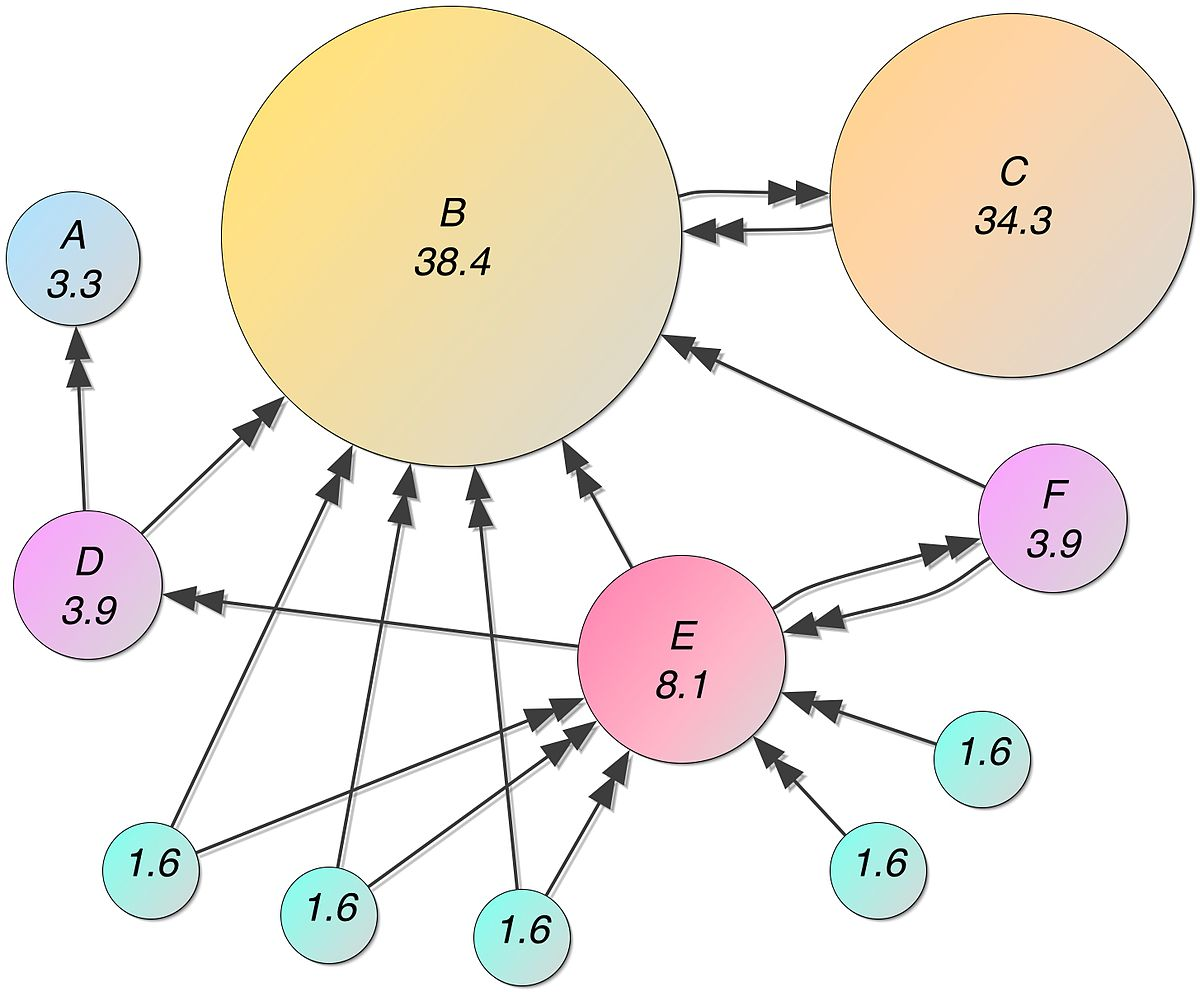
\includegraphics[width=\linewidth]{images/pagerank.jpg}
  \caption{Rappresentazione grafica del ranking con PageRank}
\end{figure}
Dal punto di vista matematico il PageRank di una pagina è definito in modo ricorsivo e dipende dal numero e dalla metrica PageRank di tutte le pagine che la collegano (archi entranti). Una pagina a cui sono collegate molte pagine con un PageRank elevato riceve un livello elevato.
\subsection{Storia}
Larry Page e Sergey Brin, i due co-fondatori di Google, svilupparono l'algoritmo PageRank nel 1996 come parte di un progetto di ricerca dell'università di Standford riguardo un nuovo tipo di motore di ricerca. Fu proprio di Sergey Brin l'idea che il World Wide Web dovesse essere ordinato per popolarità data dai link: più una pagina esiste come link nelle altre pagine, più questa deve avere un punteggio alto in classifica.

\subsection{Formulazione}
Sia $ V = \{ 1, 2, 3, \ldots \} $ un insieme di nodi.

\subsection{Tecnica}
Si propone di seguito la tecnica proposta il calcolo dello score per la classificazione degli autori. \\
La tecnica consiste nel calcolo del PageRank dei nodi utilizzando, come pesi degli archi, il numero di citazioni prima e lo stesso numero di citazioni moltiplicato per un coefficiente peggiorativo. Una volta ottenuti questi due punteggi, la loro combinazione attraverso una funzione permette di ottenere il risultato finale.
\par
Il procedimento illustrato si compone dei seguenti passi:
\begin{lstlisting}[keepspaces=true]
  1)  Definizione della matrice dei pesi p(i, j)
  
  2)  Per ogni nodo i:
        Calcolo del pagerank P(i) con pesi p 

  3)  Calcolo della nuova matrice dei pesi 
      pmod(i, j) = p(i, j) * (1 - c(i, j))
      
  4)  Per ogni nodo i:
        Calcolo del pagerank Pmod(i) con pesi pmod
        
  5)  Per ogni nodo i:
        Calcolo dello score s(i) = log(Pmod(i)) - log(P(i))
\end{lstlisting}


\begin{enumerate}
  \item 
  Al primo passo della metodologia si calcola la matrice dei pesi del PageRank. \\
  Per ogni coppia di nodi $ (i, j) $, $ p_{ij} $ sarà uguale al numero di citazioni del nodo $ i $ ad articoli scritti dal nodo $ j $. 
  \item
  Si calcola poi il PageRank: 
  \[
  P_k(i) = 
    \begin{cases} 
      \displaystyle \frac{1}{n} & k = 1 \\
      \displaystyle \frac
        {\displaystyle \sum_{j=1}^{n} p_{ji}}
        {\displaystyle \sum_{t=1}^{n} {\sum_{j=1}^{n} p_{jt}}}
        P_{k-1}(j) & k > 1 

    \end{cases} 
  \]
  dove $ k $ è il numero di iterazioni necessarie alla convergenza dell'algoritmo. L'algoritmo, basato sul metodo delle potenze (\textit{power iteration}), parte da un'approssimazione iniziale, in cui è assegnata probabilità eguale a tutti i nodi. Ad ogni iterazione aggiorna le probabilità calcolando un'approssimazione più accurata rispetto a quella dell'iterazione precedente.
  \par
  Il criterio di arresto classico dell'algoritmo consiste nella stima del miglioramento della soluzione tra l'iterazione $k$-esima e l'iterazione $k-1$-esima; ovvero nella valutazione della norma 1 tra il vettore dei PageRank all'iterazione $k$-esima e quello all'iterazione precedente:
  \[
    \Delta^{(k)} = \Arrowvert P^{(k)} - P^{(k+1)}\Arrowvert
  \]
  Quando tale valore risulta essere sotto una certa soglia, si può considerare l'algoritmo giunto a convergenza.
  \par
  All'atto pratico spesso si preferisce stabilire a priori il numero di iterazioni che l'algoritmo dovrà svolgere. Questa è la scelta fatta da Neo4J e Apache Spark all'atto di implementare l'algoritmo di PageRank.
  \item
  Si passa poi a calcolare la nuova matrice di pesi per il calcolo del PageRank modificato. L'obiettivo è limitare la modifica dell'algoritmo alla sola matrice dei pesi, in modo da lasciare inalterato l'algoritmo.
  \par
  In questo caso il peso dell'arco da un generico nodo $i$ ad un generico nodo $j$ è calcolato tenendo conto, oltre che del numero di citazioni del nodo $i$ ad articoli scritti dal nodo $j$, dell'indice di collaborazione tra i due autori e del numero di citazioni considerando il verso opposto, ovvero le citazioni del nodo $j$ ad articoli scritti dal nodo $i$. \\
  Questi parametri non sono considerati in senso assoluto. Bensì vengono considerati rapportati alle relazioni che il nodo citato ha con altri autori.
  Il generico peso è definito come segue:
  \[
    p_{ij} = 
    \left( 
      \frac
      {\displaystyle cit_{ji}}
      {\displaystyle \sum_{t=1}^{n} {cit_{jt}}}
    \right)
    \bullet
    \left(
      1 - 
      \left(
      \alpha_1
      \frac
      {\displaystyle cit_{ij}}
      {\displaystyle \sum_{s=1}^{n} {cit_{is}}}
      +
      \alpha_2
      \frac
      {\displaystyle coa_{ij}}
      {\displaystyle \sum_{s=1}^{n} {coa_{is}}}
      \right)
    \right)
  \]
  
  Nella formula sopra riportata si può notare come si effettuino due diverse normalizzazioni per la parte classica del peso $p_{ij}$ e per la parte che tiene conto dell'indice di collaborazione. Il numero di citazioni dell'arco entrante
\end{enumerate}

\section{L'implementazione}
Per l'implementazione finale è stata fatta la scelta di utilizzare un implementazione custom dell'algoritmo PageRank e dei suoi derivati. \\
Tale scelta è stata dettata dal fatto che il livello di prestazioni ottenibili utilizzando le basi di dati a grafo non erano ragionevoli per eseguire il lavoro sulla mole di dati a disposizione.
\subsection{Il linguaggio Scala}
L'implementazione è stata svolta nel linguaggio di programmazione Scala. \\
Il linguaggio Scala, linguaggio staticamente tipato basato sulla Java Virtual Machine, offre, oltre ad una sintassi espressiva e conveniente, strutture dati che rendono semplice il calcolo parallelo; calcolo parallelo molto utile per ridurre notevolmente i tempi di calcolo nelle macchine multicore.
\subsection{La generazione del grafo}
Per la generazione del grafo a partire dalla versione filtrata e compattata del dataset si è utilizzato un metodo multi-fase.
\begin{enumerate}
  \item In primo luogo è stato necessario ottenere gli autori distinti e ordinati. L'ordinamento è necessario per l'utilizzo dell'algoritmo di ricerca binaria. Per ottenere gli autori distinti e ordinati si è, in un primo momento, utilizzata una struttura dati TreeSet, struttura dati che naturalmente mantiene l'ordinamento degli oggetti. Una volta inserite le stringhe contenenti i nomi degli autori nel TreeSet è sufficiente convertire l'insieme in un array per risolvere il problema. In un secondo momento si è optato per una soluzione più efficiente. Costruendo prima un ArrayBuilder (struttura dati che mantiene un array dinamicamente crescente per la costruzione degli array), calcolando i distinti (operazione che dietro le quinte costruisce un HashSet mutabile e lo riempie) ed infine applicando l'algoritmo quickSort per ordinare l'array. Questa ottimizzazione ottiene un miglioramento delle performance di quasi un ordine di grandezza.
  \begin{lstlisting}[keepspaces=true]
def authorsArray(file: Array[Line], numLines: Int):
    Array[String] = {
  def builder(): mutable.ArrayBuilder[String] = {
    val res = mutable.ArrayBuilder.make[String]()
      cfor(0)(_ < numLines, _ + 1) { i =>
        val line = file(i)
        for (author <- line.authors) {
          res += author
        }
      }
    res
  }
  val authors = builder().result.distinct
  util.Sorting.quickSort(authors)
  authors
}    
  \end{lstlisting}
  \item Una volta ottenuti gli autori distinti il passo successivo è stato quello di 
\end{enumerate}
\end{document}
